
\documentclass[tikz,border=5pt]{standalone}

% Core packages
\usepackage{amsmath,amssymb}
\usepackage{tikz}
\usepackage{tikz-cd}
\usepackage{pgfplots}
\usepackage{multicol}
\usepackage{xcolor}
\usepackage{caption}
\usepackage{float}
\usepackage{kotex}

% TikZ / PGF configuration
\usetikzlibrary{
  arrows.meta,
  calc,
  positioning,
  shapes.geometric,
  shapes.symbols,
  fit,
  backgrounds,
  patterns,
  matrix,
  intersections,
  decorations.pathmorphing,
  decorations.markings,
  angles,
  quotes
}
\pgfplotsset{compat=1.18}

% Reusable TikZ styles
\tikzset{
  >=stealth,
  line cap=round,
  line join=round,
  every picture/.style={line width=0.9pt},
  box/.style={draw, rounded corners, minimum width=2.8cm, minimum height=1.2cm, align=center},
  circlebox/.style={draw, circle, minimum size=1cm, align=center},
  arrow/.style={->, thick},
  dashedarrow/.style={->, thick, dashed},
  point/.style={circle, fill, inner sep=1.2pt},
  gridhelp/.style={help lines, gray!35},
  highlight/.style={fill=blue!10, draw=blue!60!black},
  3D/.style={
    x={(-0.60cm,-0.42cm)},
    y={(0.78cm,0cm)},
    z={(0cm,0.78cm)}
  }
}


\begin{document}

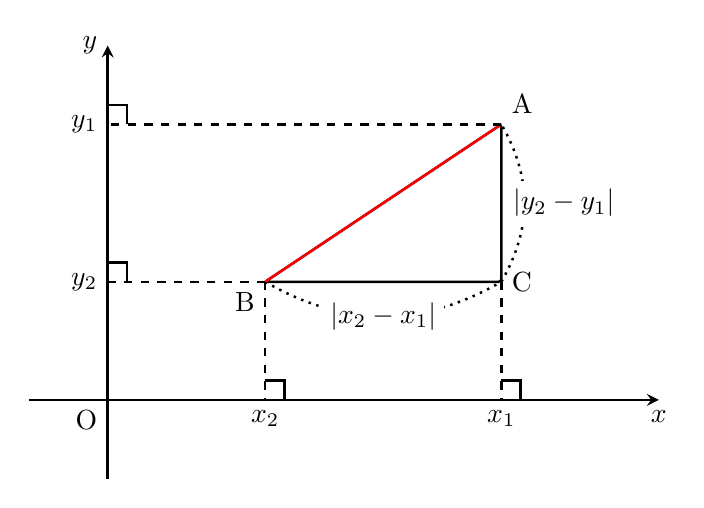
\begin{tikzpicture}[scale=1,x=10mm,y=10mm]
		\coordinate (B) at(2,1.5);
		\coordinate (C) at(5,1.5);
		\coordinate (A) at(5,3.5);
		\coordinate (C1) at(5,0);
		\coordinate (A2) at(0,3.5);
		\coordinate (B1) at(2,0);
		\coordinate (B2) at(0,1.5);

		\draw[-stealth] (-1,0)--(7,0) node[below]{$x$};
		\draw[-stealth] (0,-1)--(0,4.5) node[left]{$y$};
		\draw[rounded corners=1pt] (A)--(B)--(C)--cycle;

    \draw[dotted] (B) to[bend right=30] node[midway]{\colorbox{white}{$\left|x_2-x_1\right|$}} (C);
		\draw[dotted] (C) to[bend right=30] node[midway,xshift=5mm]{\colorbox{white}{$\left|y_2-y_1\right|$}} (A);

    \draw[color=red] (A)--(B);
		\draw[dashed] (A)--(A2) node[left]{$y_1$};
		\draw[dashed] (B)--(B1) node[below]{$x_2$};
		\draw[dashed] (B)--(B2) node[left]{$y_2$};
		\draw[dashed] (C)--(C1) node[below]{$x_1$};

    \coordinate (X) at(7,0);
    \coordinate (Y) at(0,4.5);
    \pic[draw, angle radius=7pt]{right angle = A--A2--Y};
    \pic[draw, angle radius=7pt]{right angle = B--B2--Y};
    \pic[draw, angle radius=7pt]{right angle = X--B1--B};
    \pic[draw, angle radius=7pt]{right angle = X--C1--C};

    \node[below left] at(0,0) {$\mathrm{O}$};
		\node[above right] at(A) {$\mathrm{A}$};
		\node[below left] at(B) {$\mathrm{B}$};
		\node[right] at(C) {$\mathrm{C}$};
	\end{tikzpicture}

\end{document}

